\documentclass[../main.tex]{subfiles}

\begin{document} %%%%%%%%%%%%%%%%%%%%%%%%%%%%%%%%%%%%%%%%%%%%%%%%%%%%%%%%%%%%
\section{Graficos Python}

    \begin{figure}[ht]
        \centering
        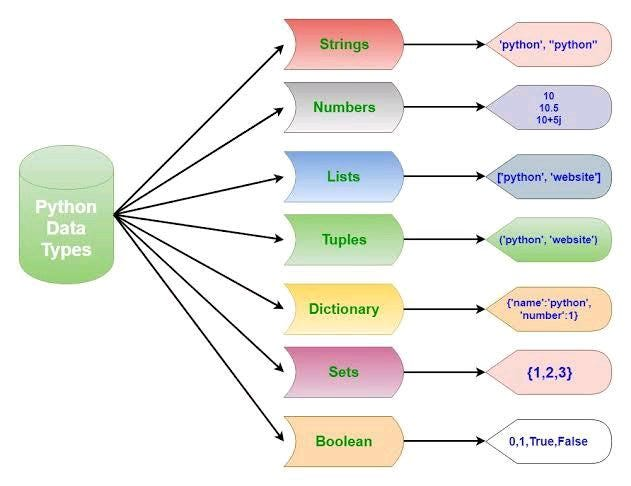
\includegraphics[width=0.85\textwidth]{./images/variables_python.jpg}
        \caption{Tipos de variables en Python}
        \label{fig:tipos_variables_python}
    \end{figure}
   
    Tipos de gráficos:
    \begin{enumerate}
        \item torta: plt.pie
        \item barras: plt.bar
        \item lineas: plt.plot
        \item scatterplot: plt.scatter o sns.scatterplot
    \end{enumerate}

    \subsection{Groupy}
        \begin{figure}[ht]
            \centering
            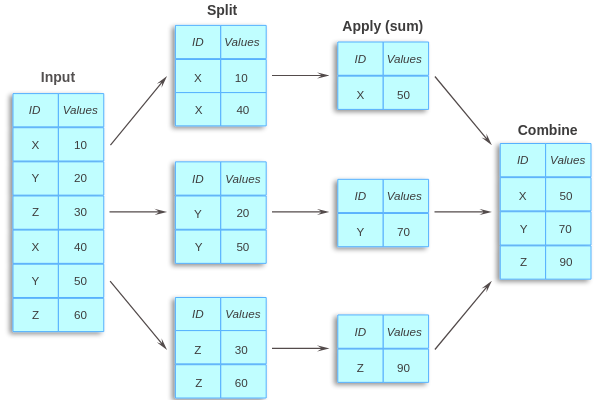
\includegraphics[width=0.85\textwidth]{./images/groupby.png}
            \caption{Groupy}
            \label{fig:groupy}
        \end{figure}

    Ver video \cite{Pandas_Split_Apply_Combine}
\end{document}  %%%%%%%%%%%%%%%%%%%%%%%%%%%%%%%%%%%%%%%%%%%%%%%%%%%%%%%%%%%%%